% ============================================================
%  MAIN — Relazione Progetto Introduzione alla Prog. Web
%  A.A. 2025-2026
% ============================================================
% ============================================================
%  PREAMBLE — Relazione Progetto Introduzione alla Prog. Web
% ============================================================

% --- Classe documento ---
\documentclass[12pt, a4paper, oneside]{article}

% --- Encoding & lingua ---
\usepackage[T1]{fontenc}
\usepackage[utf8]{inputenc}
\usepackage[italian]{babel}

% --- Font ---
\usepackage{lmodern}
\usepackage[patch=none]{microtype}

% --- Geometria pagina ---
\usepackage[
  top=2.5cm, bottom=2.5cm,
  left=3cm,  right=3cm,
  headheight=15pt
]{geometry}

% --- Intestazione e piè di pagina ---
\usepackage{fancyhdr}
\pagestyle{fancy}
\fancyhf{}
\fancyhead[L]{\small\textit{Relazione Progetto — Introduzione alla Programmazione per il Web}}
\fancyhead[R]{\small\textit{A.A.\ 2025--2026}}
\fancyfoot[C]{\thepage}
\renewcommand{\headrulewidth}{0.4pt}

% --- Colori ---
\usepackage[dvipsnames, table]{xcolor}
\definecolor{primary}{RGB}{30, 80, 160}      % blu accademico
\definecolor{secondary}{RGB}{90, 90, 90}     % grigio testo secondario
\definecolor{codebg}{RGB}{245, 245, 245}     % sfondo listati

% --- Hyperref (ultima, salvo eccezioni) ---
\usepackage[
  colorlinks = true,
  linkcolor  = primary,
  urlcolor   = primary,
  citecolor  = primary,
  pdftitle   = {Relazione Progetto Web},
  pdfauthor  = {Team},
  pdfsubject = {Introduzione alla Programmazione per il Web},
]{hyperref}

% --- Grafici e diagrammi ---
\usepackage{graphicx}
\usepackage{float}
\usepackage{tikz}
\usetikzlibrary{shapes.geometric, arrows.meta, positioning, fit, backgrounds, calc}
\usepackage{pgf-umlsd}          % diagrammi di sequenza (opzionale)

% --- Tabelle ---
\usepackage{booktabs}
\usepackage{tabularx}
\usepackage{multirow}
\usepackage{array}

% --- Listati di codice ---
\usepackage{listings}
\lstset{
  backgroundcolor = \color{codebg},
  basicstyle      = \ttfamily\small,
  keywordstyle    = \color{primary}\bfseries,
  commentstyle    = \color{secondary}\itshape,
  stringstyle     = \color{BrickRed},
  numbers         = left,
  numberstyle     = \tiny\color{secondary},
  stepnumber      = 1,
  numbersep       = 8pt,
  frame           = single,
  framerule       = 0.4pt,
  rulecolor       = \color{secondary!40},
  breaklines      = true,
  captionpos      = b,
  tabsize         = 2,
}

% --- Matematica ---
\usepackage{amsmath, amssymb}

% --- Enumerazioni personalizzate ---
\usepackage{enumitem}
\setlist[itemize]{leftmargin=1.5em, topsep=4pt, itemsep=2pt}
\setlist[enumerate]{leftmargin=1.5em, topsep=4pt, itemsep=2pt}

% --- Caption ---
\usepackage{caption}
\captionsetup{
  font        = small,
  labelfont   = {bf, color=primary},
  labelsep    = period,
  skip        = 6pt,
}

% --- Spaziatura ---
\usepackage{setspace}
\setstretch{1.15}
\setlength{\parskip}{6pt}
\setlength{\parindent}{0pt}

% --- Titolo sezione personalizzato ---
\usepackage{titlesec}
\titleformat{\section}
  {\large\bfseries\color{primary}}
  {\thesection.}{0.6em}{}[\titlerule]
\titleformat{\subsection}
  {\normalsize\bfseries\color{primary!80}}
  {\thesubsection.}{0.5em}{}
\titleformat{\subsubsection}
  {\normalsize\itshape\color{secondary}}
  {\thesubsubsection.}{0.5em}{}

\titlespacing{\section}{0pt}{14pt}{6pt}
\titlespacing{\subsection}{0pt}{10pt}{4pt}

% --- Riquadro informativo ---
\usepackage{tcolorbox}
\tcbuselibrary{skins, breakable}
\newtcolorbox{infobox}[1][]{
  enhanced,
  colback  = primary!5,
  colframe = primary!50,
  fonttitle= \bfseries,
  title    = {#1},
  breakable,
}

% --- Utility ---
\usepackage{lipsum}   % testo segnaposto — rimuovere nella versione finale
\usepackage{xspace}
\newcommand{\mvc}{\textsc{mvc}\xspace}
\newcommand{\teamid}[1]{\textbf{#1}}


\begin{document}

% ---- FRONTESPIZIO -----------------------------------------------
\begin{titlepage}
  \centering
  \vspace*{1.5cm}

  {\Large\bfseries Università degli Studi\par}
  \vspace{0.3cm}
  {\large Corso di Laurea in Informatica\par}
  \vspace{0.3cm}
  {\normalsize Insegnamento: Introduzione alla Programmazione per il Web\par}

  \vspace{1.5cm}
  \rule{\linewidth}{1.5pt}\\[0.4cm]
  {\LARGE\bfseries\color{primary} Relazione di Progetto\par}
  \vspace{0.2cm}
  {\large\itshape GymBros Centre Web App\par}
  \rule{\linewidth}{1.5pt}

  \vspace{1.2cm}
  {\large Anno Accademico 2025--2026\par}

  \vspace{1.5cm}
  \begin{tabular}{ll}
    \toprule
    \textbf{ID Team} & \teamid{07} \\
    \midrule
    \textbf{Componenti} & Stefano Videsott \\
                        & Alessandro Como \\
    % \midrule
    % \textbf{Repository} & \url{https://github.com/StefanoVidesott/project_web} \\
    \bottomrule
  \end{tabular}

  \vfill
  {\small\color{secondary} Repository del progetto disponibile a \url{https://github.com/StefanoVidesott/project_web}.\par}
  % {\small\color{secondary} Documento redatto ai fini della valutazione del progetto.\par}
\end{titlepage}

% ---- INDICE -----------------------------------------------------
% \tableofcontents
% \thispagestyle{empty}
% \newpage

% ---- SEZIONI ----------------------------------------------------
% ============================================================
%  SEZIONE 1 — Introduzione
% ============================================================
\section{Introduzione}

\subsection{Obiettivo del progetto}

% Descrivete il problema assegnato e l'obiettivo da raggiungere.
% Esempio: "Il progetto consiste nella realizzazione di un'applicazione web per la gestione di..."
[Descrivere qui il problema/obiettivo assegnato dal progetto.]

\subsection{Scelte architetturali iniziali}

% Spiegate come avete impostato le cose e perché.
[Illustrare le scelte iniziali per la definizione dell'architettura, motivando le principali decisioni progettuali.]

\subsection{Soluzioni alternative considerate}

% Riportare eventuali approcci valutati e poi scartati, con le relative motivazioni.
[Descrivere eventuali soluzioni alternative che sono state prese in considerazione e le ragioni per cui sono state poi abbandonate.]

% ============================================================
%  SEZIONE 2 — Architettura
% ============================================================
\section{Architettura}

\subsection{Pattern MVC e organizzazione del progetto}
Abbiamo adottato il pattern architetturale \mvc (Model--View--Controller),
strutturato su tre livelli distinti.

\begin{itemize}
  \item \textbf{Model.} I POJO del dominio (\texttt{User}, \texttt{Training}, \texttt{Composition}, \texttt{CustomComposition}, \texttt{Review}, \ldots) e i repository gestiscono l'accesso al database H2 tramite \texttt{JdbcTemplate}. Mapper dedicati (\texttt{UserMapper}, \texttt{TrainingMapper}, \texttt{ExerciseMapper}, \ldots) si occupano della conversione da \texttt{ResultSet} a oggetto del dominio, tenendo questa logica fuori dai repository. La gestione degli utenti di sicurezza è delegata a \texttt{JdbcUserDetailsManager}, che opera sulle tabelle \texttt{USERS} e \texttt{AUTHORITIES}.

  \item \textbf{View.} I template Thymeleaf compongono le pagine HTML. I componenti comuni, intestazione, barra di navigazione, carosello delle recensioni, footer e script Bootstrap, sono estratti come fragment riutilizzabili nella directory \texttt{templates/bases/}. Il frontend usa Bootstrap~5 per il layout e Chart.js per gli istogrammi delle statistiche; le chiamate alle recensioni usano \texttt{fetch} con \texttt{async}/\texttt{await} per aggiornare la pagina senza ricaricarla. Abbiamo scelto \texttt{async}/\texttt{await} perché rispetto a \texttt{XMLHttpRequest} o alle Promise con \texttt{.then()} il codice risulta più leggibile e segue il flusso di esecuzione in modo più lineare.

  \item \textbf{Controller.} I controller gestiscono le richieste HTTP seguendo il pattern \textbf{controller $\to$ service $\to$ repository} e sono organizzati per area funzionale (\texttt{MainController}, \texttt{AdminDashboardController}, \texttt{TrainingController},\\\texttt{ReviewController}, \ldots). I service incapsulano la logica applicativa: \texttt{CheckUserService} verifica l'unicità dello username, \texttt{PlanService} valida i piani con una whitelist dei ruoli consentiti per impedire la \textit{privilege escalation} ad amministratore, \texttt{PasswordValidationService} valida il formato della password lato server, necessario perché le validazioni JavaScript lato client possono essere aggirate modificando le richieste HTTP.
\end{itemize}

\subsection{Comunicazione tra i servizi}
La web app principale comunica con il REST service tramite OpenFeign: il client \texttt{TrainingsProxy} dichiara gli endpoint del REST service come metodi Java annotati, e il framework genera l'implementazione HTTP. Il REST service espone i programmi predefiniti, la composizione di ciascun programma e il calcolo delle calorie. %, ed è in ascolto sulla porta 8081.

\subsection{Diagramma dell'architettura}
% La Figura~\ref{fig:architettura} illustra la struttura del sistema.

\begin{figure}[H]
\centering
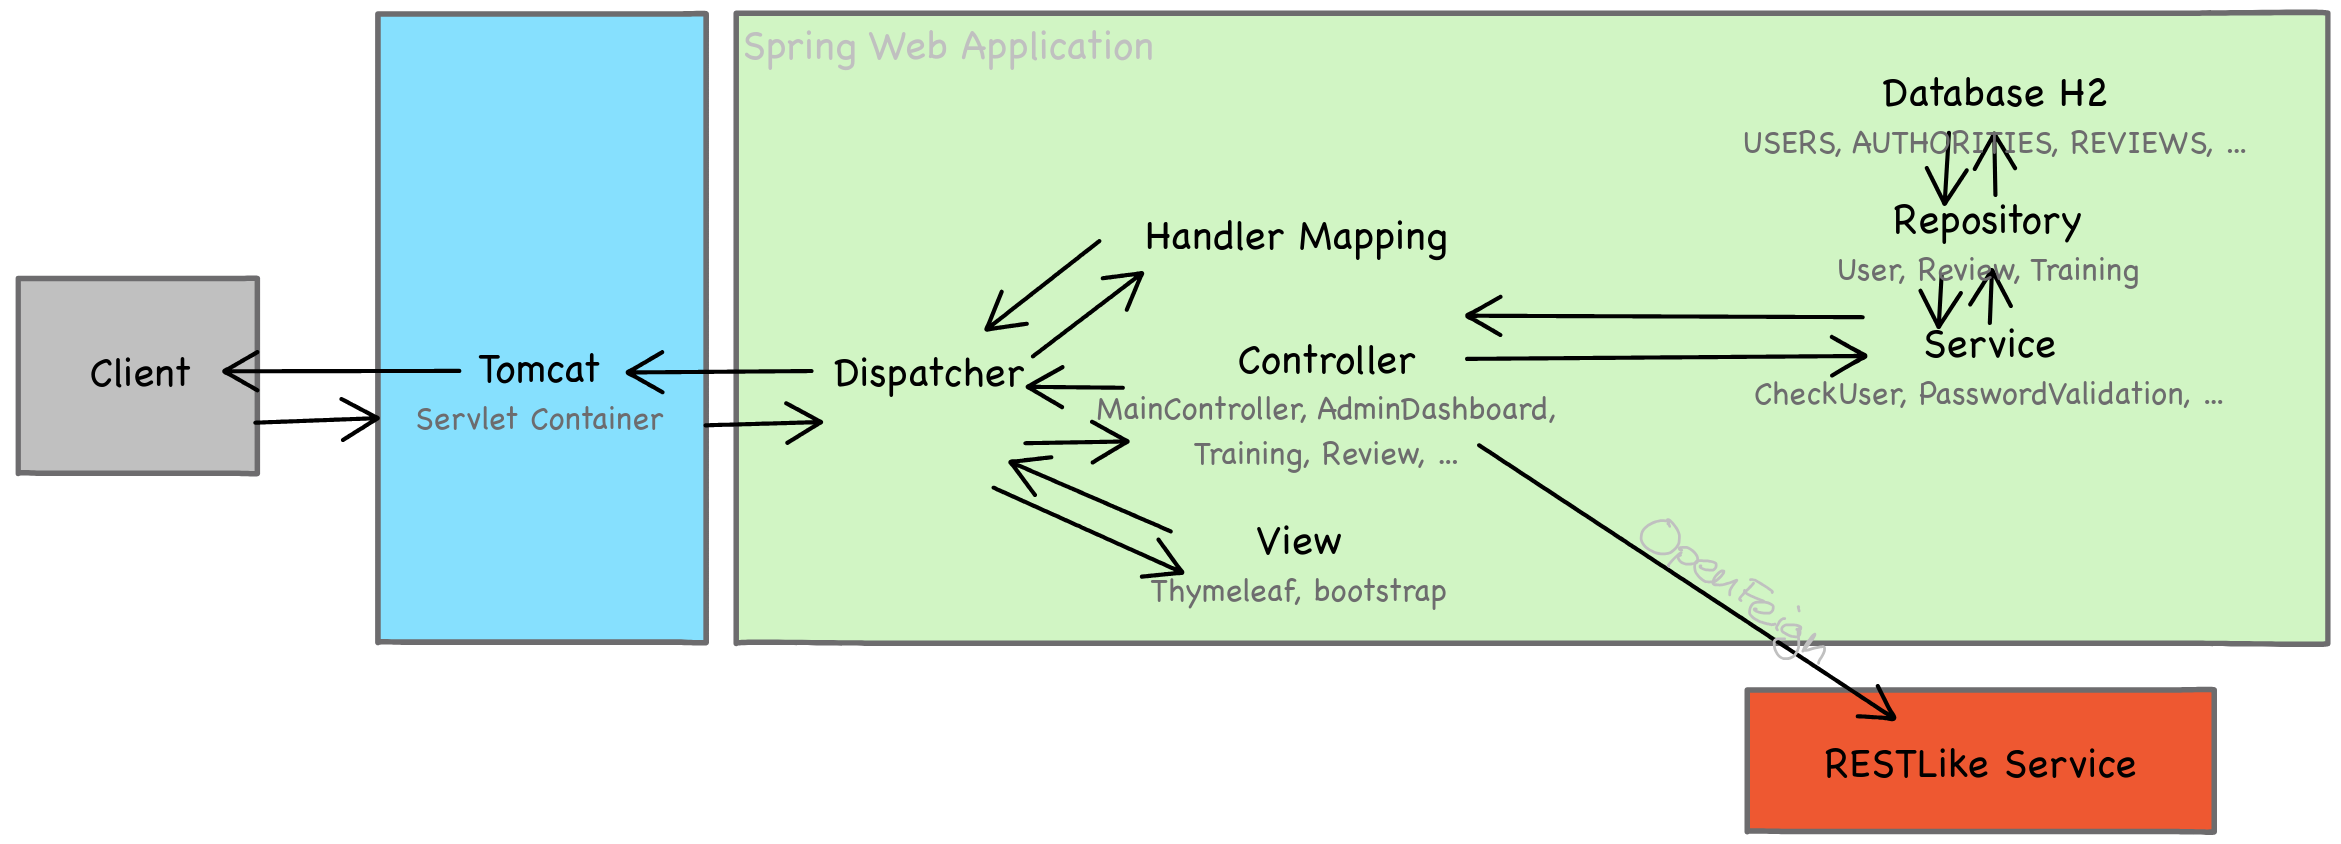
\includegraphics[width=\textwidth]{resources/architecture_schema.png}
\caption{Diagramma dell'architettura del sistema.}
\label{fig:architettura}
\end{figure}

% \begin{figure}[H]
% \centering
% \begin{tikzpicture}[
%       node distance = 0.9cm and 2cm,
%       every node/.style = {font=\small},
%       layer/.style    = {
%         draw, rounded corners=4pt, minimum width=3.2cm,
%         minimum height=1cm, align=center,
%         fill=primary!12, draw=primary!60, text=black, thick
%       },
%       arrow/.style    = {-Stealth, thick, color=primary!80},
%       dbnode/.style   = {
%         draw, cylinder, shape border rotate=90,
%         aspect=0.35, minimum width=2.2cm, minimum height=0.9cm,
%         fill=secondary!15, draw=secondary!60, align=center, font=\small
%       },
%       client/.style   = {
%         draw, rounded corners=4pt, minimum width=3.2cm,
%         minimum height=1cm, align=center,
%         fill=BrickRed!10, draw=BrickRed!50, thick
%       },
%     ]
% \node[client]  (browser) {Browser\\\textit{(Client)}};
% \node[layer,   right=of browser]  (ctrl)    {Controller\\(Routing \& Logic)};
% \node[layer,   above=of ctrl]     (view)    {View\\(Template / HTML)};
% \node[layer,   below=of ctrl]     (model)   {Model\\(Business Logic)};
% \node[dbnode,  right=of model]    (db)      {Database};
% \draw[arrow] (browser.east)  -- node[above, font=\tiny]{HTTP Request}  (ctrl.west);
% \draw[arrow] (ctrl.west)     -- node[below, font=\tiny]{HTTP Response} (browser.east);
% \draw[arrow] (ctrl.north)  -- node[right, font=\tiny]{render}  (view.south);
% \draw[arrow] (view.south)  -- node[left,  font=\tiny]{template} (ctrl.north);
% \draw[arrow] (ctrl.south)  -- node[right, font=\tiny]{call}   (model.north);
% \draw[arrow] (model.north) -- node[left,  font=\tiny]{data}   (ctrl.south);
% \draw[arrow] (model.east) -- node[above, font=\tiny]{query}  (db.west);
% \draw[arrow] (db.west)    -- node[below, font=\tiny]{result} (model.east);
% \begin{pgfonlayer}{background}
% \node[
%         draw=primary!40, dashed, rounded corners=6pt,
%         fill=primary!4,
%         fit=(ctrl)(view)(model),
%         label={[font=\footnotesize\itshape, color=primary!70]above:Server-side},
%       ] {};
% \end{pgfonlayer}
% \end{tikzpicture}
% % \caption{Diagramma dell'architettura \mvc del sistema.}
% \label{fig:architettura}
% \end{figure}

% \subsection{Struttura delle directory}
% \begin{lstlisting}[language=bash, caption={Struttura del progetto dopo il refactoring.}]
% main_webapp/
% |-- src/main/java/exam_project/main_webapp/
% |   |-- configurations/    SecurityConfig, ProjectConfig,
% |   |                      MainWebappApplication
% |   |-- controllers/       AdminDashboardController, MainController,
% |   |                      PasswordController, ProfileController,
% |   |                      ReviewController, StatisticsController,
% |   |                      TrainingController, UpgradeController
% |   |-- mappers/           DefaultTrainingCountersMapper, ExerciseMapper,
% |   |                      TrainingMapper, UserMapper, UserSummaryMapper
% |   |-- pojos/             Composition, CustomComposition, ExerciseDTO,
% |   |                      Review, SecurityUser, Training, User
% |   |-- proxies/           TrainingsProxy (OpenFeign)
% |   |-- repositories/      ReviewRepository, TrainingRepository,
% |   |                      UserRepository
% |   |-- services/          CheckUserService, PasswordValidationService,
% |   |                      PlanService, ReviewService, StatisticsService,
% |   |                      TrainingService, UserService
% |-- src/main/resources/
% |   |-- templates/
% |   |   |-- bases/         head.html, navbar.html, footer.html,
% |   |   |                  carosello.html, review.html, scripts.html
% |   |   |-- *.html         Pagine pubbliche e dashboard
% |   |-- static/
% |   |   |-- css/           style.css
% |   |   |-- js/            review.js, customTraining.js,
% |   |                      changePassword.js, signup.js,
% |   |                      loginValidation.js, carosello.js
% |   |-- application.properties
% |   |-- schema.sql
% |   |-- data.sql

% RestLike/
% |-- src/main/java/org/example/restlike/
% |   |-- Controllers/       MainController
% |   |-- Mappers/           CompositionRowMapper, ExerciseRowMapper,
% |   |                      TrainingRowMapper
% |   |-- Pojos/             Composition, Exercise, Training
% |   |-- Repository/        TrainingRepository
% |-- src/main/resources/
%     |-- schema.sql
%     |-- data.sql
% \end{lstlisting}

% ============================================================
%  SEZIONE 3 — Funzionalità
% ============================================================
\section{Funzionalità}

\subsection{Descrizione della funzionalità selezionata}

% Scegliete UNA funzionalità significativa da descrivere nel dettaglio.
[Descrivere qui la funzionalità scelta, il suo scopo e il contesto d'uso all'interno dell'applicazione.]

\subsection{Interazione utente}

Dal punto di vista dell'utente, la funzionalità si articola nei seguenti passi:

\begin{enumerate}
  \item Passo 1: descrivere l'azione dell'utente.
  \item Passo 2: descrivere la risposta del sistema.
  \item Passo 3: eventuale feedback o esito finale.
\end{enumerate}

\subsection{Flusso interno al sistema}

La Figura~\ref{fig:sequenza} mostra il diagramma di sequenza relativo all'esecuzione della funzionalità, evidenziando i componenti coinvolti e i messaggi scambiati.

\begin{figure}[H]
  \centering
  % --- Diagramma di sequenza con TikZ ---
  \begin{tikzpicture}[
      actor/.style  = {draw, thick, fill=primary!10, minimum width=2.2cm,
                       minimum height=0.7cm, rounded corners=3pt,
                       font=\small\bfseries, align=center},
      lifeline/.style = {draw, dashed, thick, color=secondary!60},
      msg/.style    = {-Stealth, thick, color=primary!80},
      retmsg/.style = {-Stealth, dashed, thick, color=secondary},
      lbl/.style    = {font=\scriptsize, fill=white, inner sep=1pt},
    ]

    % --- Attori (asse X) ---
    \def\xBrowser{0}
    \def\xCtrl{3.5}
    \def\xModel{7}
    \def\xDB{10.5}

    \node[actor] (A) at (\xBrowser, 0) {Browser};
    \node[actor] (B) at (\xCtrl,    0) {Controller};
    \node[actor] (C) at (\xModel,   0) {Model};
    \node[actor] (D) at (\xDB,      0) {Database};

    % --- Lifelines ---
    \foreach \x in {\xBrowser, \xCtrl, \xModel, \xDB}{
      \draw[lifeline] (\x, -0.35) -- (\x, -5.8);
    }

    % --- Messaggi (asse Y scende) ---
    % 1. Request
    \draw[msg] (\xBrowser,-0.8) -- node[lbl,above]{1. HTTP Request} (\xCtrl,-0.8);
    % 2. validate & fetch
    \draw[msg] (\xCtrl,-1.4) -- node[lbl,above]{2. [validate] fetch()} (\xModel,-1.4);
    % 3. query
    \draw[msg] (\xModel,-2.0) -- node[lbl,above]{3. SQL query} (\xDB,-2.0);
    % 4. result set
    \draw[retmsg] (\xDB,-2.6) -- node[lbl,above]{4. result set} (\xModel,-2.6);
    % 5. domain object
    \draw[retmsg] (\xModel,-3.2) -- node[lbl,above]{5. domain object} (\xCtrl,-3.2);
    % 6. render view
    \draw[msg] (\xCtrl,-3.8) -- node[lbl,above]{6. render(view, data)} (\xBrowser+0.3,-3.8);
    % piccola freccia interna al controller per indicare passaggio alla view
    \draw[msg] (\xCtrl,-4.4) -- node[lbl,above]{7. View populated} (\xCtrl+0.01,-4.4);
    % 8. HTTP Response
    \draw[retmsg] (\xCtrl,-5.2) -- node[lbl,above]{8. HTTP Response (HTML)} (\xBrowser,-5.2);

  \end{tikzpicture}
  \caption{Diagramma di sequenza della funzionalità selezionata.}
  \label{fig:sequenza}
\end{figure}

\subsection{Funzionalità non implementate}

% Descrivere eventuali funzionalità previste ma non realizzate, con motivazione.
[Elencare e motivare le funzionalità che non è stato possibile implementare, specificando se si tratta di vincoli temporali, tecnici o di altra natura.]

% ============================================================
%  SEZIONE 4 — Criticità e sviluppi futuri
% ============================================================
\section{Criticità della soluzione e sviluppi futuri}

\subsection{Problemi incontrati durante lo sviluppo}

% Descrivere i principali ostacoli tecnici o organizzativi affrontati.
[Descrivere i principali problemi incontrati nel corso dello sviluppo, specificando le cause e come sono stati affrontati.]

\subsection{Limiti della soluzione attuale}

% Indicare in modo onesto i limiti tecnici o funzionali dell'applicazione consegnata.
[Illustrare i limiti noti della soluzione, ad esempio in termini di scalabilità, sicurezza, copertura dei casi d'uso o qualità del codice.]

\subsection{Possibili miglioramenti futuri}

Tra i possibili sviluppi futuri si identificano:

\begin{itemize}
  \item Miglioramento 1: descrivere brevemente.
  \item Miglioramento 2: descrivere brevemente.
  \item Miglioramento 3: descrivere brevemente.
\end{itemize}

% ============================================================
%  SEZIONE 5 — Contributo dei componenti del gruppo
% ============================================================
\section{Contributo di ogni componente del gruppo}
% La Tabella~\ref{tab:contributi} riassume le attività svolte da ciascun
% componente del team.

\begin{table}[H]
\centering
% \caption{Ripartizione del lavoro tra i membri del team.}
\label{tab:contributi}
\renewcommand{\arraystretch}{1.3}
\begin{tabularx}{\linewidth}{l X}
\toprule
\textbf{Componente} & \textbf{Attività svolte} \\
\midrule
\textbf{Stefano Videsott} &
  Architettura iniziale della web app principale; Spring Security,
  controller, service layer e repository; parte del frontend frontend (relativo alle parti sviluppate), autenticazione e registrazione, dahsboards con alcune delle funzionalità, logica legata alle recensioni con
  \texttt{fetch}/\texttt{async}/\texttt{await}; statistiche Chart.js;
  refactoring completo finale della codebase per
  uniformare i contributi di entrambi i membri (nomi di classi,
  metodi, variabili, tabelle e colonne DB rinominati in inglese con
  convenzioni coerenti). \\
\textbf{Alessandro Como} &
  Realizzazione della homepage e della pagina di contatto. Progettazione e sviluppo del REST service: controller, repository,
  schema SQL e dati di test; integrazione con OpenFeign REST;
  buisness logic e view relative alla visualizzazione e al completamento degli allenamenti e delle parti collegate. \\
\bottomrule
\end{tabularx}
\end{table}

La prima parte di ideazione e modellazione dello schema del database è stata fatta insieme.

% ============================================================
%  SEZIONE 6 — Lezioni apprese
% ============================================================
\section{Lezioni apprese}

\subsection{Aspetti tecnici}
Abbiamo innanzitutto imparato le basi di Spring, un framework che nessuno di noi due aveva mai utilizzato; abbiamo imparato ad impostare correttamente la parte di secuirity per gestire correttamente authorization e authentication. Abbiamo inoltre consolidato concetti della programmazione asincrona, che avevamo già visto nel corso di \textit{Ingegneria del Software} e che in questo corso abbiamo capito davvero.

\subsection{Aspetti progettuali}
Sviluppare in parallelo sulla stessa applicazione ci ha permesso, al termine del lavoro, di renderci conto che è utile concordare dei pattern di sviluppo e delle convenzioni di naming, senza le quali ci si trova ad avere del codice eterogeneo e dispersivo.

\subsection{Cosa rifaremmo diversamente}
Avremmo definito lo schema del database e le convenzioni di naming prima di iniziare: ogni modifica a progetto completato ha richiesto tempo per la comprenzione e adeguare il codice in modo uniforme, operazione ripetuta troppe volte nella fase di refactor che ha richiesto diverse ore. Per il frontend useremmo una libreria differente per avere un frontend meno vincolato dalla logica dei dati oppure quantomeno Tailwind CSS al posto di Bootstrap, per avere un look più moderno e facile da scrivere.

\subsection{Risorse aggiuntive}
Nel corso del progetto sono state consultate diverse risorse esterne,
in particolare per la realizzazione del frontend. Le principali sono:

\begin{itemize}
  \item Baeldung, textit{thymeleaf-extras-springsecurity6}:
    \url{https://www.baeldung.com/spring-security-thymeleaf}

  \item Documentazione ufficiale Bootstrap~5: componenti carousel, navbar,
    tabelle, alert, radio toggle buttons, layout dei form e utility di
    sizing e spacing @
    \url{https://getbootstrap.com/docs/5.3/}

  \item W3Schools, Bootstrap navbar e form @
    \url{https://www.w3schools.com/bootstrap5/bootstrap_navbar.php},
    \url{https://www.w3schools.com/bootstrap/bootstrap_forms.asp}

  \item Colorlib, template login di riferimento per il layout delle
    pagine di accesso @
    \url{https://colorlib.com/wp/template/login-form-11/}

  \item MDN Web Docs, template literals JavaScript @
    \url{https://developer.mozilla.org/en-US/docs/Web/JavaScript/Reference/Template_literals}

  \item Stack Overflow, formattazione decimali in Thymeleaf e
    centratura elementi con Bootstrap @
    \url{https://stackoverflow.com/questions/52132580},
    \url{https://stackoverflow.com/questions/42388989}

  \item chart.js @ \url{https://www.chartjs.org/}
\end{itemize}

\end{document}
